% Relatório do TP "Analisando Grafos do SNAP" -- G13 soc-RedditHyperlinks
% Overleaf: abra o template WebMedia ("Open as Template"), envie esta pasta inteira
% (main.tex, referencias.bib, valores.tex, tabelas/, figuras/) e compile main.tex.
% Sem o webmedia.cls (ex.: compilação local), cai para o acmart, no qual ele é baseado.
\PassOptionsToPackage{expansion=false}{microtype} % evita erro com fontes não escaláveis em instalações locais
\IfFileExists{webmedia.cls}{\documentclass[sigconf]{webmedia}}{\documentclass[sigconf]{acmart}}

\usepackage[brazilian]{babel}
\usepackage{graphicx}
\usepackage{booktabs}
\usepackage{array}
\usepackage{adjustbox}
\usepackage[section]{placeins} % figuras e tabelas não passam para depois da seção seguinte
% caracteres Unicode que aparecem nas tabelas geradas
\DeclareUnicodeCharacter{2260}{\ensuremath{\neq}}
\DeclareUnicodeCharacter{00B3}{\textsuperscript{3}}
\DeclareUnicodeCharacter{00B2}{\textsuperscript{2}}
\DeclareUnicodeCharacter{00B7}{\ensuremath{\cdot}}
\DeclareUnicodeCharacter{2192}{\ensuremath{\rightarrow}}
\DeclareUnicodeCharacter{2248}{\ensuremath{\approx}}
\DeclareUnicodeCharacter{2265}{\ensuremath{\geq}}
\DeclareUnicodeCharacter{2264}{\ensuremath{\leq}}
\DeclareUnicodeCharacter{2212}{\ensuremath{-}}
\DeclareUnicodeCharacter{03B3}{\ensuremath{\gamma}}
\DeclareUnicodeCharacter{2309}{\ensuremath{\rceil}}
\DeclareUnicodeCharacter{2308}{\ensuremath{\lceil}}
\DeclareUnicodeCharacter{2079}{\textsuperscript{9}}
\graphicspath{{figuras/}}
% Gerado por src/relatorio.py (escrever_macros). Não editar à mão.
\newcommand{\matricula}{224216276}
\newcommand{\grafoID}{13}
\newcommand{\postsTotal}{286.561}
\newcommand{\nVertices}{35.776}
\newcommand{\nArestas}{124.330}
\newcommand{\nArestasDir}{137.821}
\newcommand{\grauMax}{2.336}
\newcommand{\grauMedio}{6{,}95}
\newcommand{\densidade}{$1{,}94 \times 10^{-4}$}
\newcommand{\nComponentes}{497}
\newcommand{\nLCC}{34.671}
\newcommand{\mLCC}{123.570}
\newcommand{\fracLCC}{96{,}9\%}
\newcommand{\diametro}{11}
\newcommand{\raio}{6}
\newcommand{\caminhoMedio}{3{,}91}
\newcommand{\clustMedio}{0{,}181}
\newcommand{\transitividade}{0{,}0584}
\newcommand{\nTriangulos}{406.391}
\newcommand{\linksNeg}{21.070}
\newcommand{\fracNeg}{7{,}4\%}
\newcommand{\nSCC}{24.071}
\newcommand{\maiorSCC}{11.564}
\newcommand{\fracSCC}{32{,}3\%}
\newcommand{\nPontes}{18.057}
\newcommand{\nArticulacoes}{5.006}
\newcommand{\pesoAGM}{25.435{,}5}
\newcommand{\iterBFmin}{8}
\newcommand{\iterBFmax}{10}
\newcommand{\tBFS}{32{,}9}
\newcommand{\tDijkstra}{134}
\newcommand{\tBF}{409}
\newcommand{\tFWmil}{1{,}9}
\newcommand{\tFWpuroQuinhentos}{4{,}68}
\newcommand{\tFWQuinhentos}{0{,}211}
\newcommand{\razaoC}{865}
\newcommand{\razaoL}{0{,}706}
\newcommand{\sigmaER}{1.225{,}3}
\newcommand{\Caleat}{$2{,}15 \times 10^{-4}$}
\newcommand{\Laleat}{5{,}55}
\newcommand{\razaoCgraus}{4{,}28}
\newcommand{\razaoLgraus}{1{,}05}
\newcommand{\sigmaGraus}{4{,}08}
\newcommand{\Cgraus}{0{,}0435}
\newcommand{\Lgraus}{3{,}73}
\newcommand{\gammaBruto}{1{,}44}
\newcommand{\rBruto}{0{,}861}
\newcommand{\gammaBins}{2{,}11}
\newcommand{\rBins}{0{,}992}
\newcommand{\gammaCCDF}{2{,}32}
\newcommand{\gammaMLE}{2{,}22}
\newcommand{\kminMLE}{31}
\newcommand{\rRemover}{1.734}
\newcommand{\Srand}{0{,}924}
\newcommand{\SrandDP}{0{,}00457}
\newcommand{\crand}{869}
\newcommand{\Sgrau}{0{,}366}
\newcommand{\cgrau}{17.458}
\newcommand{\Lgrau}{12{,}1}
\newcommand{\isoGrau}{48{,}6\%}
\newcommand{\Sbtw}{0{,}364}
\newcommand{\cbtw}{17.799}
\newcommand{\Lbtw}{8{,}7}
\newcommand{\Spr}{0{,}428}
\newcommand{\cpr}{16.176}
\newcommand{\Lpr}{6{,}69}
\newcommand{\Lorig}{3{,}92}
\newcommand{\Lrand}{3{,}92}
\newcommand{\isoRand}{2{,}5\%}
\newcommand{\reciprocidade}{19{,}6\%}
\newcommand{\concNeg}{39{,}0\%}
\newcommand{\topIndegree}{askreddit}
\newcommand{\topNeg}{subredditdrama}
\newcommand{\nucleos}{2}
\newcommand{\tDist}{243}


\settopmatter{printacmref=false, printfolios=false}
\setcopyright{none}
\renewcommand\footnotetextcopyrightpermission[1]{}
\acmConference{}{}{}
\acmDOI{}
\acmISBN{}

% ------------------------------------------------------------------ autor (preencher)
\newcommand{\autorNome}{Edwu}                 % TODO: nome completo
\newcommand{\autorEmail}{email@ufba.br}       % TODO: e-mail
\newcommand{\repo}{\url{https://github.com/RottyWheels/Analise-de-Dados-com-Grafo-do-Sub-reddit}}

\begin{document}

\title{Conflito e centralidade entre comunidades do Reddit}
\subtitle{Análise do grafo G13 (\texttt{soc-RedditHyperlinks}) do SNAP}

\author{\autorNome}
\email{\autorEmail}
\affiliation{%
  \institution{Instituto de Computação, Universidade Federal da Bahia}
  \city{Salvador}
  \state{BA}
  \country{Brasil}}
\renewcommand{\shortauthors}{\autorNome}

\begin{abstract}
Este trabalho analisa a rede de hiperlinks entre subreddits do Reddit (\texttt{soc-RedditHyperlinks},
SNAP), atribuída pela matrícula \matricula{} (grafo G\grafoID). A partir de \postsTotal{} posts com link
entre 2014 e 2017, construímos um grafo estático com \nVertices{} subreddits e \nArestas{} arestas,
calculamos suas medidas estruturais, implementamos e medimos os algoritmos da disciplina e investigamos
as propriedades de mundo pequeno, lei de potência e robustez. A rede é de mundo pequeno
(diâmetro \diametro, caminho médio \caminhoMedio), tem distribuição de graus de cauda pesada
($\gamma \approx \gammaMLE$) e é robusta a falhas aleatórias, mas frágil a ataques: remover os 5\% de
maior grau reduz a maior componente a \Sgrau{} do tamanho original. Código, dados tratados e
resultados estão em \repo.
\end{abstract}

\keywords{teoria dos grafos, redes complexas, Reddit, mundo pequeno, lei de potência, robustez}

\maketitle

% =================================================================================
\section{Introdução}
Redes sociais on-line se organizam em comunidades que se citam, cooperam e entram em conflito.
No Reddit, cada comunidade é um \emph{subreddit}, e um post que cita outro subreddit cria uma relação
dirigida entre os dois. \citet{kumar2018} reuniram esses hiperlinks e rotularam cada um como positivo
ou negativo (hostil), conforme o tom do post. O resultado, disponível no SNAP~\cite{snap}, é um grafo
dirigido, temporal e com sinal.

Este relatório aplica os conceitos da disciplina a esse grafo: tratamento dos dados, medidas
estruturais (Parte~I), implementação e análise de complexidade de algoritmos clássicos (Parte~II) e
investigação de propriedades de redes complexas (Parte~III). Todas as medidas e algoritmos são
implementações próprias, testadas contra o NetworkX.

% =================================================================================
\section{Determinação do Grafo}
A regra do enunciado é
$f(M) = ((\text{soma dos dígitos de } M) \times (\text{últimos 2 dígitos de } M + 1)) \bmod 129$,
usando 129 quando o resultado é 0. Para $M = 224216276$:
\begin{itemize}
  \item soma dos dígitos: $2+2+4+2+1+6+2+7+6 = 32$;
  \item últimos dois dígitos: $76$, logo $76 + 1 = 77$;
  \item $(32 \times 77) \bmod 129 = 2464 \bmod 129 = 13$.
\end{itemize}
O grafo atribuído é o \textbf{G13, \texttt{soc-RedditHyperlinks}} (categoria \emph{Social networks}).
O mesmo conjunto de dados aparece na planilha também como G72 (\emph{Signed}), G92 (\emph{Temporal}) e
G109 (\emph{Online communities}); usamos a entrada G13, indicada pela regra.

% =================================================================================
\section{Código e Dados}
O repositório \repo{} contém o código (\texttt{src/}), os testes (\texttt{tests/}, 44 testes com o
NetworkX como referência), o notebook que executa todos os experimentos, os dados tratados
(\texttt{data/processed/}), as figuras e as tabelas. O \texttt{README} explica a instalação e a
execução; \texttt{scripts/run\_all.py} reproduz tudo sem abrir o Jupyter, e
\texttt{scripts/verificar\_dados.py} confere o arquivo baixado contra as contagens esperadas.

% =================================================================================
\section{Descrição do Grafo Original}
O SNAP distribui dois arquivos: hiperlinks no corpo dos posts (\emph{body}) e no título (\emph{title}).
Usamos o arquivo \emph{body}, com \postsTotal{} linhas. Cada linha registra o subreddit de origem, o de
destino, o identificador do post, a data, o sinal do link ($+1$ ou $-1$) e um vetor de 86 atributos
de texto. O período vai de 31/12/2013 a 30/04/2017. Há \linksNeg{} links negativos (\fracNeg). A
Figura~\ref{fig:original} mostra o volume mensal de posts e a proporção dos sinais.

Os números da planilha da disciplina (55.863 vértices e 858.490 arestas) descrevem o conjunto completo,
somando \emph{body} e \emph{title}; por isso diferem dos nossos.

\begin{figure}[t]
  \centering
  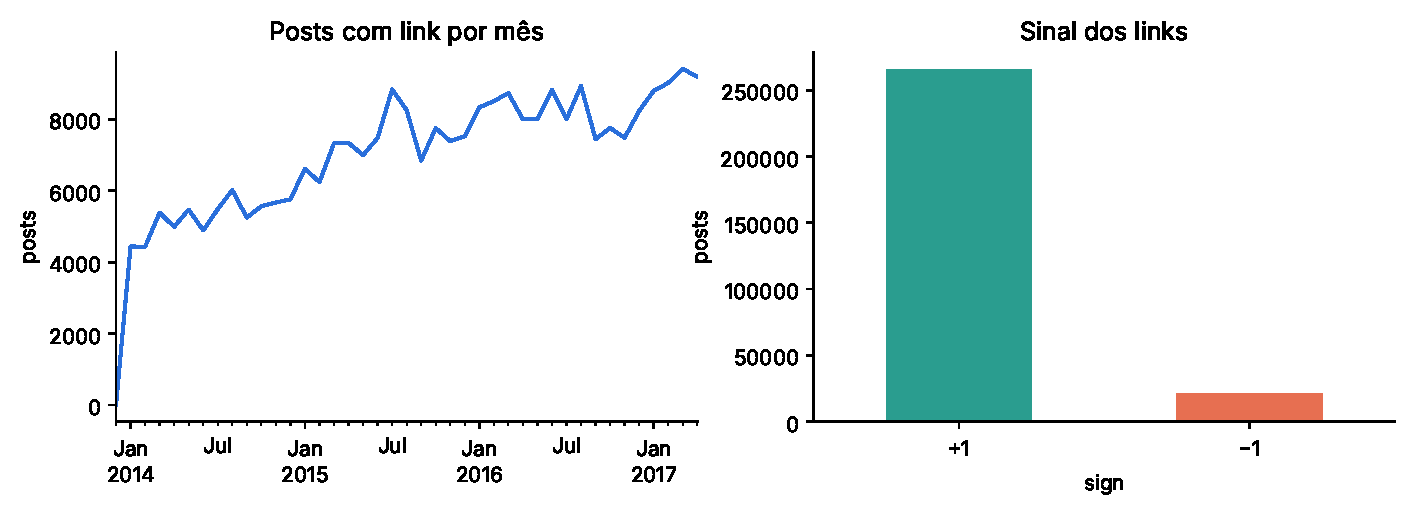
\includegraphics[width=\linewidth]{01_original_tempo_sinal.pdf}
  \caption{Posts com hiperlink por mês e proporção dos sinais no arquivo original.}
  \label{fig:original}
\end{figure}

% =================================================================================
\section{Tratamento dos Dados}
A Tabela~\ref{tab:tratamento} resume os tratamentos. Os principais foram:
\begin{enumerate}
  \item \textbf{Temporal $\rightarrow$ estático:} união de todos os posts do período.
  \item \textbf{Multigrafo $\rightarrow$ simples:} uma aresta por par $(u \rightarrow v)$, com
    \texttt{count} (nº de posts) e \texttt{sign} (sinal majoritário). O grafo dirigido tem
    \nArestasDir{} arestas.
  \item \textbf{Dirigido $\rightarrow$ não dirigido:} $u \rightarrow v$ e $v \rightarrow u$ viram uma
    aresta, com contagens somadas: \nArestas{} arestas. O grafo dirigido foi mantido para Tarjan,
    Euler dirigido e PageRank.
  \item \textbf{Pesos:} $w = 1/\texttt{count}$, para que pares com mais links fiquem mais próximos.
    São pesos reais, não sintéticos.
  \item \textbf{Maior componente conexa:} \nLCC{} vértices (\fracLCC) e \mLCC{} arestas, usada nas
    medidas de distância, no small-world e na robustez.
\end{enumerate}
O arquivo não tem auto-laços. Descartamos o vetor de atributos de texto, que não é usado nas
análises e ocupa a maior parte dos 319~MB do arquivo.

\begin{table*}[t]
\centering
\small
\caption{Tratamentos aplicados ao arquivo original.}
\label{tab:tratamento}
\begin{adjustbox}{max width=\linewidth}
\begin{tabular}{lll}
\toprule
Tratamento & Descrição & Resultado \\
\midrule
Temporal → estático & União de todos os posts de 31/12/2013 a 30/04/2017 & 286.561 posts \\
Remoção de auto-loops & Verificado: o arquivo não tem auto-loops & 0 removidos \\
Multigrafo → simples (dirigido) & Uma aresta por par (u→v); count = nº de posts; sign = sinal majoritário & 137.821 arestas \\
Dirigido → não dirigido & Junta u→v e v→u; count somado; sign pelo saldo ponderado & 124.330 arestas \\
Pesos & w = 1/count (pares com mais links ficam mais próximos) & Dijkstra, Bellman-Ford, Floyd-Warshall, AGM \\
Maior componente conexa & Usada em distâncias, small-world e robustez & 34.671 vértices / 123.570 arestas \\
Subgrafos de teste & Subgrafos induzidos conexos por BFS (n = 100 a 16.000) & Floyd-Warshall e curvas de tempo \\
Atributos descartados & Vetor PROPERTIES (86 atributos de texto) e POST\_ID & economia de memória \\
\bottomrule
\end{tabular}
\end{adjustbox}
\end{table*}


% =================================================================================
\section{Metodologia}
\textbf{Implementação.} O código é Python~3 com listas de adjacência em dicionários. Pandas é usado
para ler os dados e o NetworkX apenas para montar o grafo e conferir resultados nos testes; o igraph
confere, de forma opcional, as distâncias e o betweenness exatos. Os algoritmos seguem
\citet{cormen2009} e \citet{tarjan1972}.

\textbf{Distâncias.} Diâmetro, raio e caminho médio são exatos: uma BFS a partir de cada um dos
\nLCC{} vértices da maior componente, distribuídas entre \nucleos{} núcleos (\tDist~s no total).

\textbf{Tempo de execução.} Cada medição tem uma execução de aquecimento descartada e roda com o
coletor de lixo do Python desligado. No grafo completo, cada algoritmo roda 30 vezes, com origens
sorteadas; com $n \geq 30$, o intervalo de confiança de 95\% é $\bar{x} \pm z_{\alpha/2}\,s/\sqrt{n}$.
Para a complexidade observada, medimos subgrafos conexos de tamanho crescente (coletados por BFS),
com 10 repetições por tamanho e IC pela t-Student ($n < 30$), e ajustamos o tempo médio a
$c \cdot f(n,m)$ por mínimos quadrados.

\textbf{Small-world, lei de potência e robustez.} Seguimos os apêndices do enunciado. O grafo
aleatório de referência é um $G(n,m)$ gerado por código próprio~\cite{erdos1959}; acrescentamos um
segundo nulo, que preserva a sequência de graus por trocas duplas de arestas~\cite{maslov2002}.
O expoente $\gamma$ é estimado por regressão linear em escala log-log e por máxima
verossimilhança~\cite{clauset2009}. Na robustez, removemos $r = \lceil 0{,}05\,n \rceil = \rRemover$
vértices ao acaso (30 repetições) ou os de maior centralidade, com ranking fixo, por grau,
betweenness (algoritmo de \citet{brandes2001} com 1.000 fontes sorteadas~\cite{brandes2007}) e
PageRank~\cite{page1999}.

% =================================================================================
\section{Resultados}

\subsection{Parte I: análise estrutural}
A Tabela~\ref{tab:parte1} reúne as medidas; todas foram calculadas. O grafo é muito esparso
(densidade \densidade) e quase conexo: a maior componente concentra \fracLCC{} dos vértices, e as
outras \nComponentes{} componentes são, em sua maioria, pares ou trios de subreddits isolados.
O grau médio é \grauMedio, mas o máximo chega a \grauMax{} (\texttt{askreddit}): a distribuição de graus
(Figura~\ref{fig:graus}) é muito assimétrica.

Apesar do tamanho, a rede é compacta: diâmetro \diametro, raio \raio{} e caminho médio
\caminhoMedio{} na maior componente. A clusterização média é \clustMedio{}, com \nTriangulos{}
triângulos. A transitividade global (\transitividade) é bem menor que a clusterização média, sinal de
que os triângulos se concentram em vértices de grau baixo, enquanto os hubs ligam vizinhos que não se
conectam entre si. A Figura~\ref{fig:visual} mostra o núcleo da rede.

\begin{table*}[t]
\centering
\small
\caption{Parte I: medidas estruturais e indicação do que foi calculado.}
\label{tab:parte1}
\begin{adjustbox}{max width=\linewidth}
\begin{tabular}{llll}
\toprule
Medida & Valor & Grafo & Calculado? \\
\midrule
Número de vértices & 35.776 & G\_und & sim \\
Número de arestas & 124.330 & G\_und & sim \\
Grau mínimo & 1 & G\_und & sim \\
Grau máximo & 2.336 & G\_und & sim \\
Grau médio & 6,95 & G\_und & sim \\
Distribuição de graus & figura 03 & G\_und & sim \\
Densidade & $1,943 \times 10^{-4}$ & G\_und & sim \\
Número de componentes conexas & 497 & G\_und & sim \\
Tamanho de cada componente & tabela 03 & G\_und & sim \\
Tamanho da maior componente & 34.671 (96,9\%) & G\_und & sim \\
Diâmetro & 11 & maior componente & sim (exato, BFS própria) \\
Raio & 6 & maior componente & sim (exato, BFS própria) \\
Comprimento médio dos caminhos & 3,914 & maior componente & sim (exato, BFS própria) \\
Coeficiente de clusterização médio & 0,1809 & G\_und & sim \\
Transitividade (clusterização global) & 0,0584 & G\_und & sim (extra) \\
Número de triângulos & 406.391 & G\_und & sim \\
Visualização & figura 03b (versão reduzida) & top 150 por grau & sim \\
\bottomrule
\end{tabular}
\end{adjustbox}
\end{table*}


\begin{figure}[t]
  \centering
  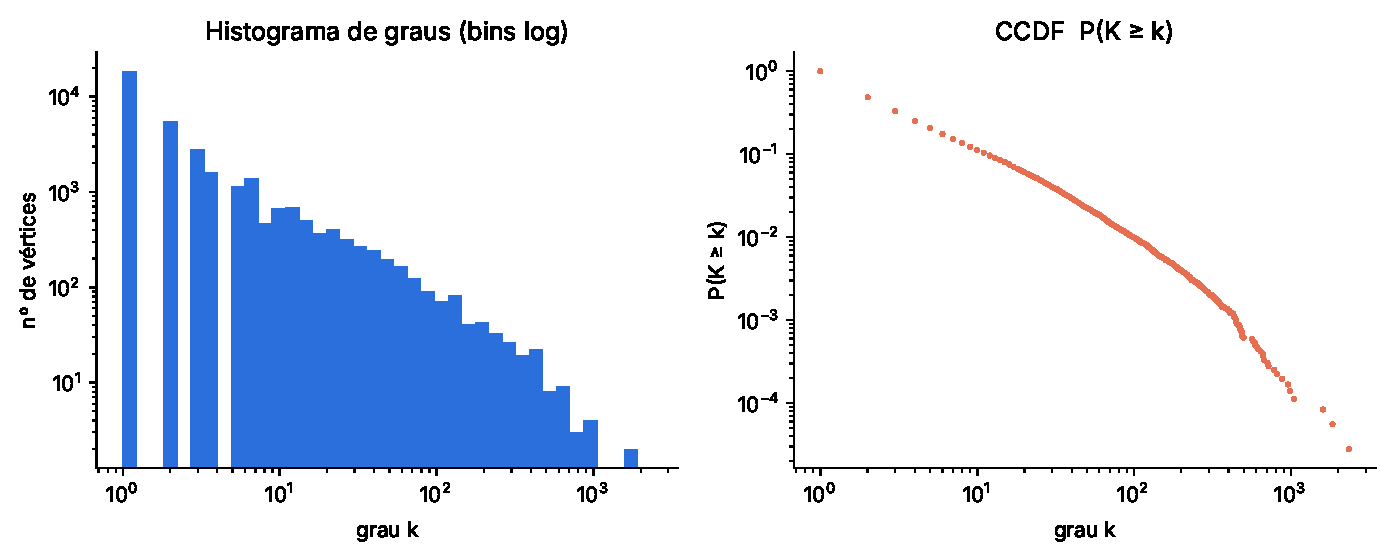
\includegraphics[width=\linewidth]{03_distribuicao_graus.pdf}
  \caption{Distribuição de graus: histograma com bins logarítmicos e CCDF.}
  \label{fig:graus}
\end{figure}

\begin{figure}[t]
  \centering
  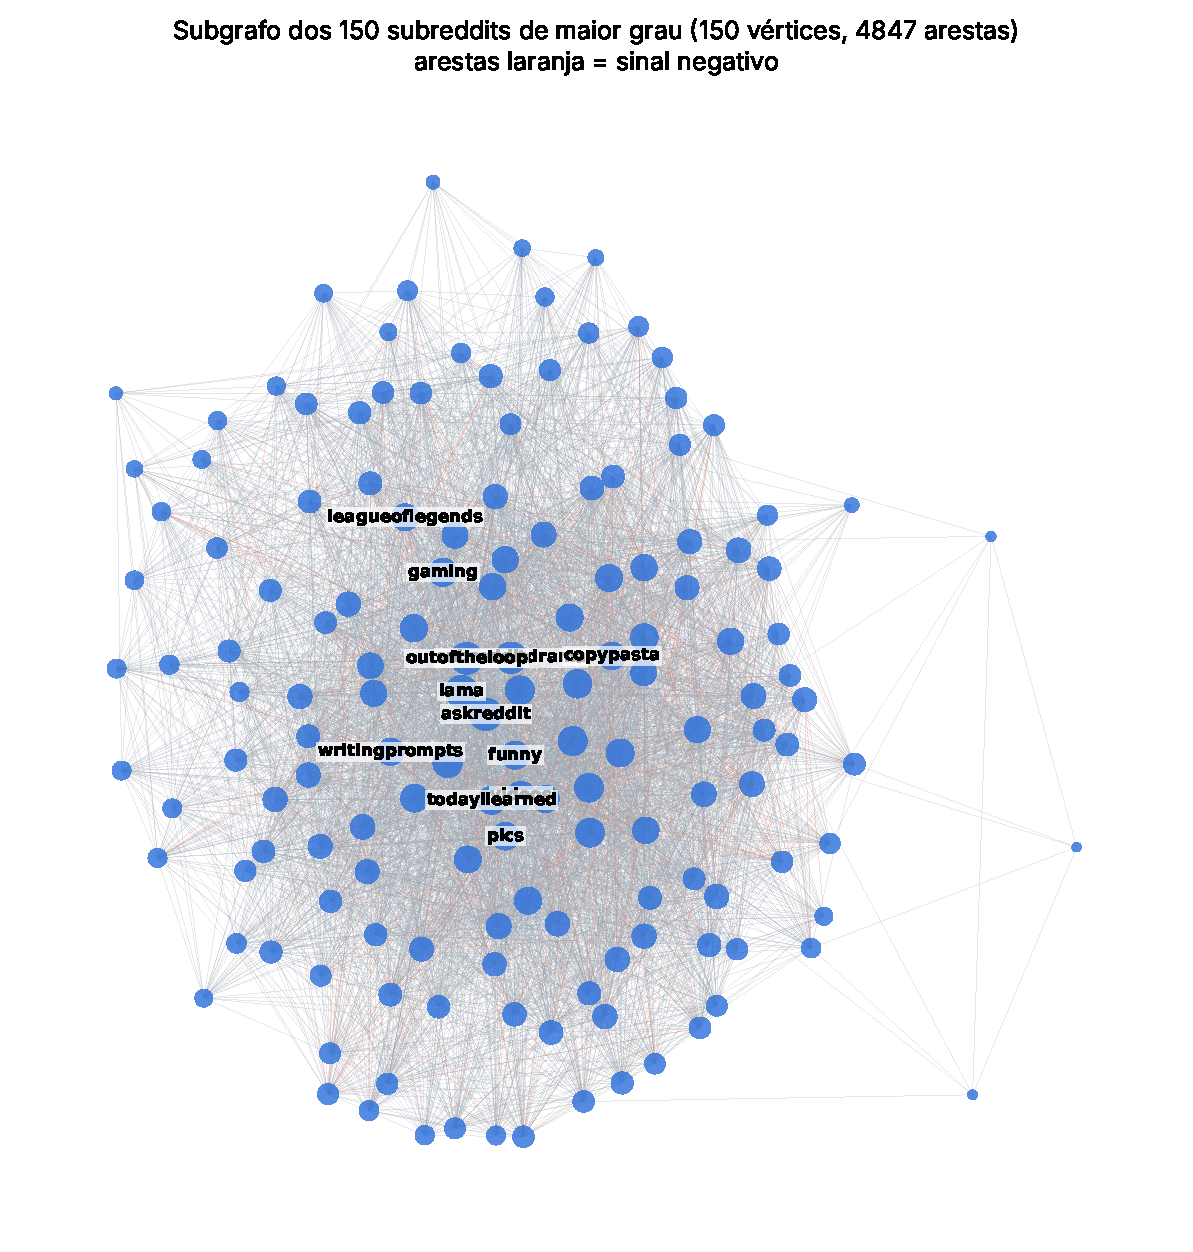
\includegraphics[width=0.9\linewidth]{03b_visualizacao.pdf}
  \caption{Subgrafo dos 150 subreddits de maior grau; arestas laranja têm sinal negativo.}
  \label{fig:visual}
\end{figure}

\subsection{Parte II: algoritmos}
A Tabela~\ref{tab:algoritmos} resume a saída de cada algoritmo e a Tabela~\ref{tab:tempos}, os tempos.
\begin{itemize}
  \item \textbf{BFS e DFS} alcançam toda a maior componente; a excentricidade de \texttt{askreddit} é
    igual ao raio.
  \item \textbf{Euler:} o grafo não é euleriano nem semieuleriano, por ser desconexo e ter milhares de
    vértices de grau ímpar; no dirigido, quase todos os vértices têm entrada diferente da saída.
  \item \textbf{Dijkstra e Bellman-Ford} dão as mesmas distâncias. Bellman-Ford convergiu em
    \iterBFmin{} a \iterBFmax{} rodadas, muito menos que as $n-1$ do pior caso, porque a implementação
    para quando uma rodada não altera nenhuma distância.
  \item \textbf{Bellman-Ford com sinal:} usando o sinal dos links como peso, há ciclos negativos,
    ou seja, ciclos de hostilidade líquida entre comunidades. Nesse caso não existe caminho mínimo bem
    definido; é o cenário em que Bellman-Ford se aplica e Dijkstra não.
  \item \textbf{Floyd-Warshall} só roda em subgrafos: no grafo inteiro, a matriz de distâncias teria
    $34.671^2 \approx 1{,}2\cdot10^9$ células (cerca de 9,6~GB). A versão vetorizada com numpy leva
    \tFWQuinhentos~s com 500 vértices, contra \tFWpuroQuinhentos~s da versão em Python puro.
  \item \textbf{Tarjan:} há \nSCC{} componentes fortemente conexas, mas a maior tem \maiorSCC{}
    vértices (\fracSCC): a maioria dos subreddits só envia ou só recebe links. Na maior componente
    não dirigida há \nPontes{} pontes e \nArticulacoes{} vértices de articulação, quase todos
    subreddits pendurados em um único vizinho.
  \item \textbf{Prim e Kruskal} produzem árvores geradoras com o mesmo peso (\pesoAGM).
\end{itemize}

\begin{table*}[t]
\centering
\small
\caption{Parte II: resultados dos algoritmos no G13.}
\label{tab:algoritmos}
\begin{adjustbox}{max width=\linewidth}
\begin{tabular}{lp{0.78\linewidth}}
\toprule
Algoritmo & Resultado \\
\midrule
BFS & origem = askreddit; alcança 34.671 vértices; excentricidade = 6 \\
DFS & origem = askreddit; visita 34.671 vértices \\
Euler (não dirigido) & 25.306 vértices de grau ímpar; conexo: não; euleriano: não; semieuleriano: não \\
Euler (dirigido) & 32.257 vértices com entrada ≠ saída; fracamente conexo: não; euleriano: não \\
Dijkstra & w = 1/count; maior distância a partir de askreddit = 4,59 \\
Bellman-Ford & mesmas distâncias que Dijkstra: sim; rodadas até convergir: 6 (10 origens: 8–10); ciclo negativo: não \\
Floyd-Warshall & só em subgrafos (n ≤ 2000): O(n³) e matriz 34.671² ≈ 1,2·10⁹ células (\textasciitilde{}9,6 GB) inviáveis \\
Tarjan (SCC) & 24.071 componentes fortemente conexas; maior = 11.564 vértices (32,3\%); 23.949 unitárias; 497 fracamente conexas \\
Tarjan (pontes e articulações) & maior componente: 18.057 pontes (14,6\% das arestas) e 5.006 vértices de articulação (14,4\%) \\
Kruskal & 34.670 arestas; peso total = 25.435,531 \\
Prim & 34.670 arestas; peso total = 25.435,531 (igual ao Kruskal: sim) \\
\bottomrule
\end{tabular}
\end{adjustbox}
\end{table*}

\begin{table*}[t]
\centering
\small
\caption{Tempo de execução: 30 repetições, IC de 95\% pela Normal ($z_{0{,}025}=1{,}96$).}
\label{tab:tempos}
\begin{adjustbox}{max width=\linewidth}
\begin{tabular}{lllrrrr}
\toprule
Algoritmo & Complexidade & Grafo & Média (ms) & Desvio (ms) & IC inf. (ms) & IC sup. (ms) \\
\midrule
BFS & O(n + m) & maior componente & 32,94 & 1,672 & 32,35 & 33,54 \\
DFS & O(n + m) & maior componente & 30,81 & 1,53 & 30,27 & 31,36 \\
Euler (não dirigido) & O(n + m) & G\_und & 51,48 & 10,19 & 47,83 & 55,13 \\
Euler (dirigido) & O(n + m) & G\_dir & 112,3 & 7,221 & 109,7 & 114,9 \\
Dijkstra & O((n + m) log n) & maior componente & 134,1 & 12,11 & 129,8 & 138,4 \\
Bellman-Ford & O(n · m) & maior componente & 409,1 & 58,86 & 388,1 & 430,2 \\
Tarjan (SCC) & O(n + m) & G\_dir & 65,84 & 3,956 & 64,42 & 67,25 \\
Tarjan (pontes e articulações) & O(n + m) & maior componente & 76,63 & 6,794 & 74,2 & 79,06 \\
Kruskal & O(m log m) & maior componente & 104,3 & 11,61 & 100,2 & 108,5 \\
Prim & O(m log n) & maior componente & 249,4 & 27,19 & 239,7 & 259,1 \\
Floyd-Warshall (n=100) & O(n³) & subgrafo n=100 & 2,505 & 0,1521 & 2,451 & 2,559 \\
Floyd-Warshall (n=250) & O(n³) & subgrafo n=250 & 21,6 & 0,8804 & 21,29 & 21,92 \\
Floyd-Warshall (n=500) & O(n³) & subgrafo n=500 & 211,1 & 17,05 & 205 & 217,2 \\
Floyd-Warshall (n=1000) & O(n³) & subgrafo n=1000 & 1.900,8 & 80,33 & 1.872,1 & 1.929,6 \\
Floyd-Warshall puro (n=100) & O(n³) & subgrafo n=100 & 27,83 & 1,825 & 27,18 & 28,49 \\
Floyd-Warshall puro (n=250) & O(n³) & subgrafo n=250 & 147,3 & 11,4 & 143,2 & 151,3 \\
Floyd-Warshall puro (n=500) & O(n³) & subgrafo n=500 & 4.677,3 & 227,2 & 4.596,0 & 4.758,6 \\
\bottomrule
\end{tabular}
\end{adjustbox}
\end{table*}


\textbf{Complexidade observada.} A Figura~\ref{fig:escala} e a Tabela~\ref{tab:ajuste} comparam o
tempo medido com a função teórica. Floyd-Warshall segue $n^3$ ($R^2 \approx 1$), e Dijkstra, Kruskal
e Prim acompanham bem suas curvas. Para os algoritmos lineares, a curva $c\,(n+m)$ se ajusta pior:
os subgrafos começam pelo núcleo denso, e a razão $m/n$ cai de cerca de 17 para 3,6 à medida que
crescem. Como, em Python, visitar um vértice custa bem mais que percorrer uma aresta, um ajuste com
custos separados, $a\,n + b\,m$, chega a $R^2 \approx 0{,}99$, compatível com $O(n+m)$. O
Bellman-Ford fica abaixo do pior caso $O(n \cdot m)$: com poucas rodadas, o custo efetivo é
$O(k \cdot m)$.

\begin{figure*}[t]
  \centering
  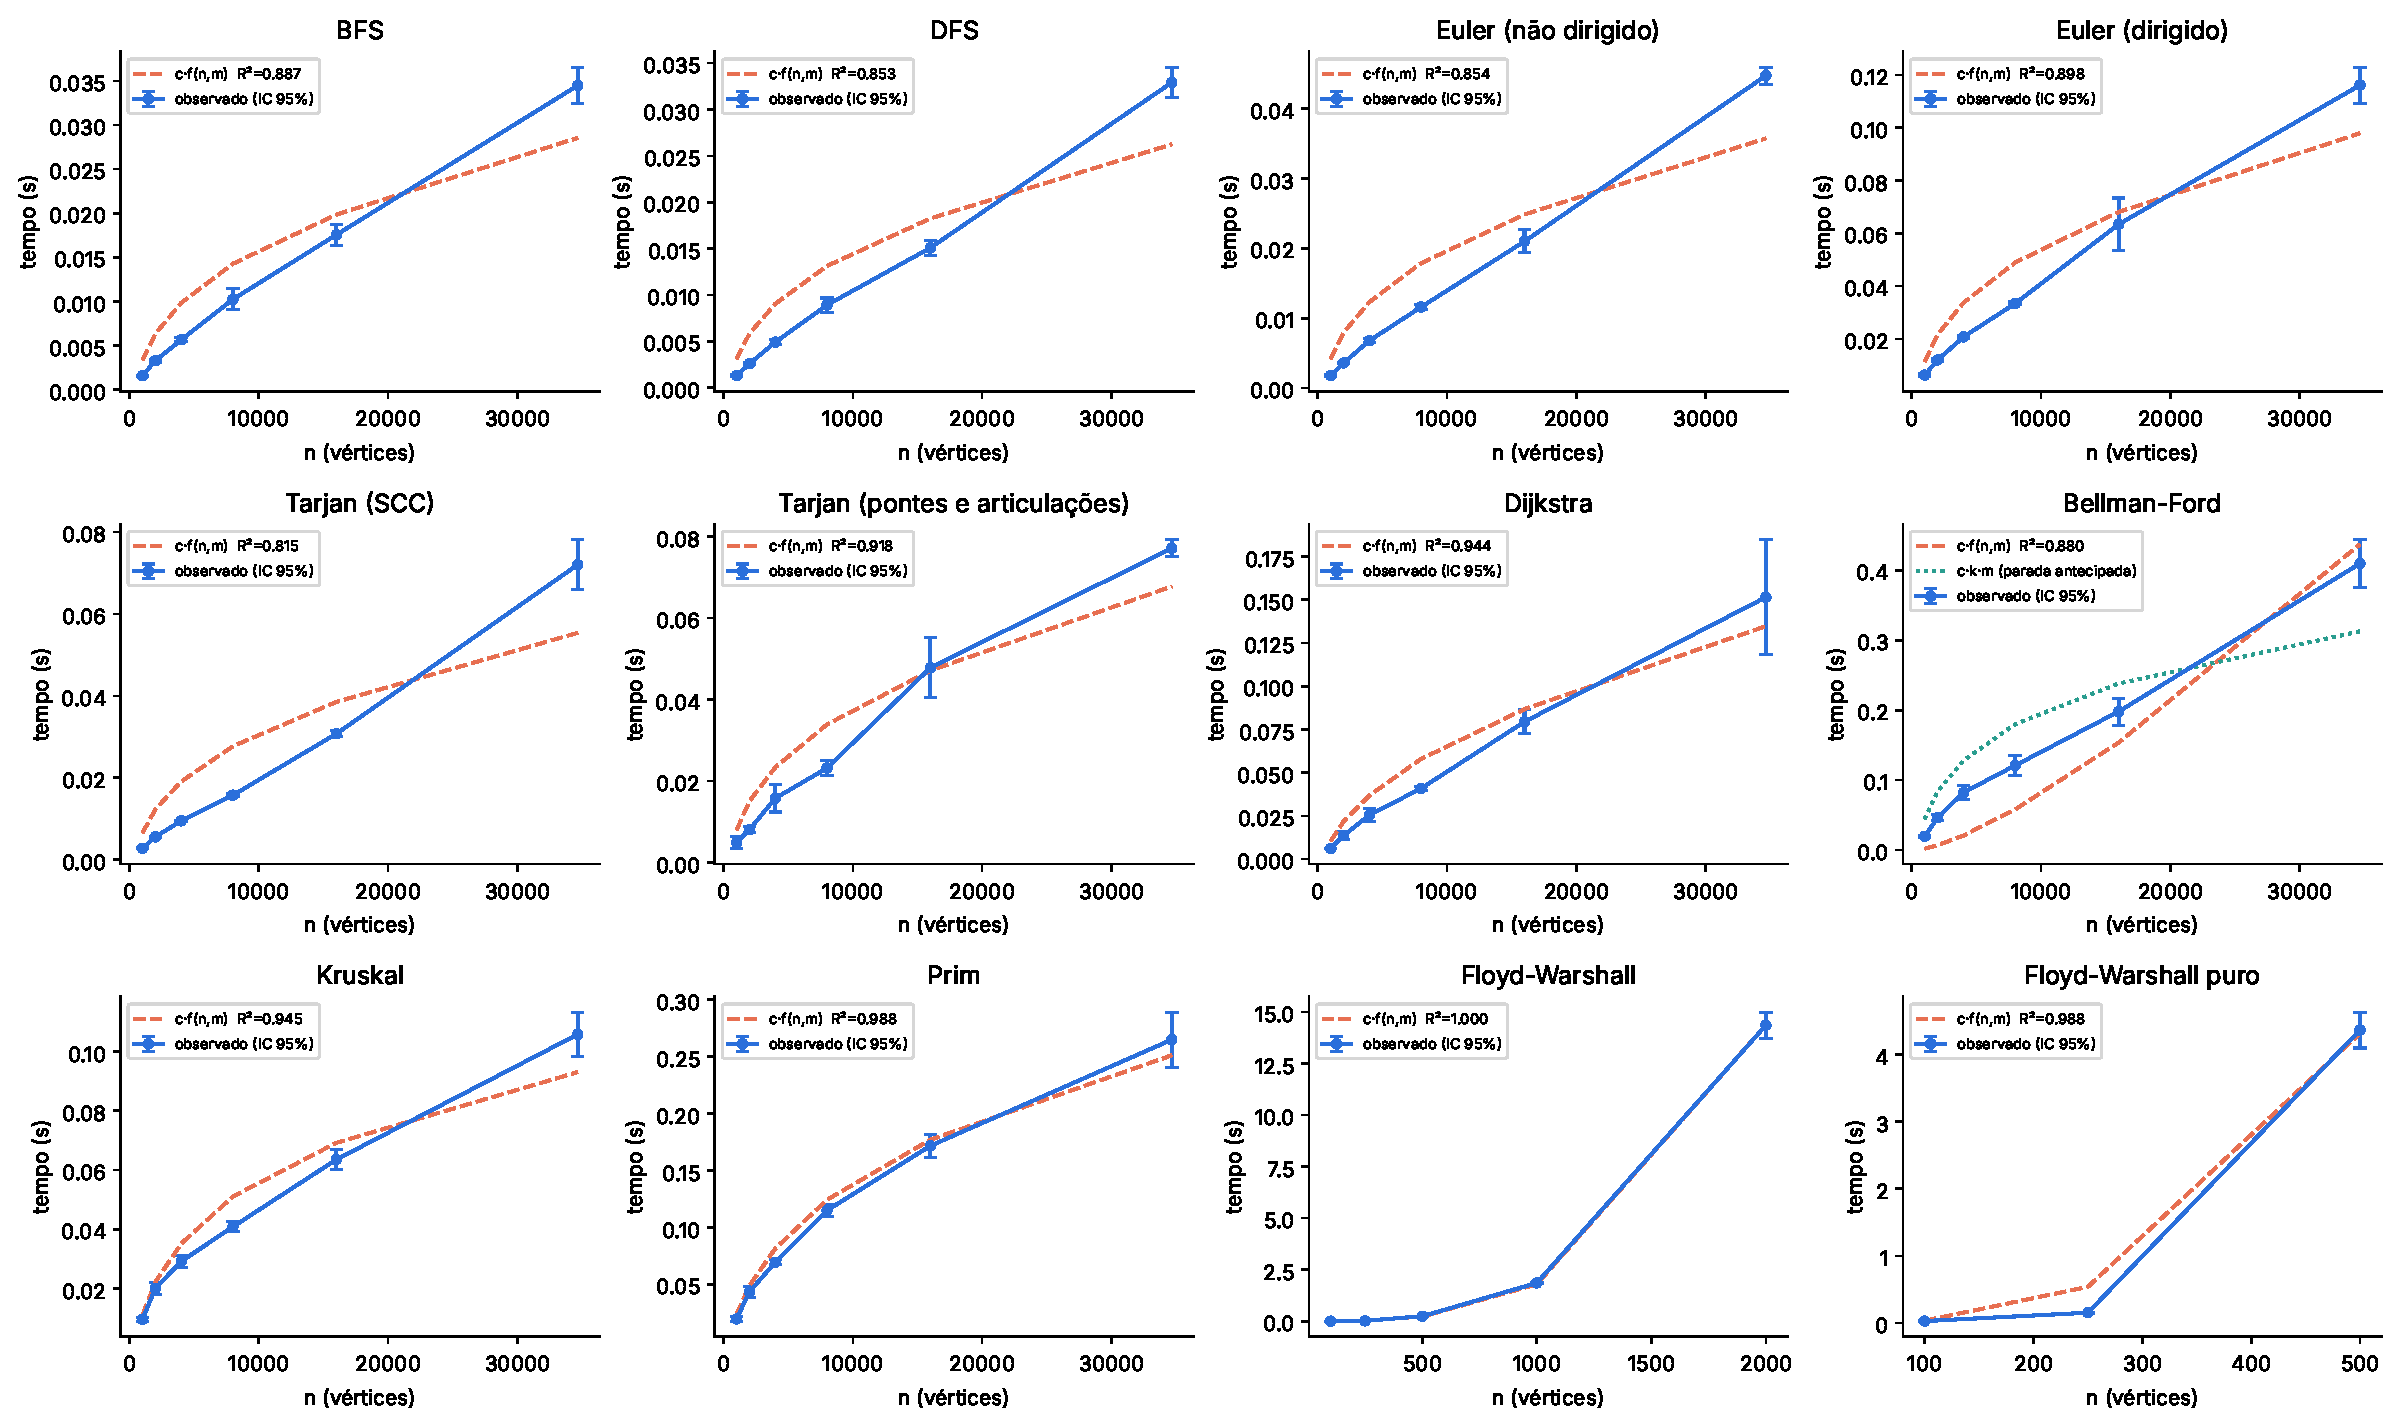
\includegraphics[width=\textwidth]{04_complexidade_observada.pdf}
  \caption{Tempo médio (IC de 95\%, t-Student) em subgrafos crescentes e curva teórica ajustada.}
  \label{fig:escala}
\end{figure*}

\begin{table}[t]
\centering
\small
\caption{Complexidade observada: ajuste do tempo médio a $c \cdot f(n,m)$ e a $a n + b m$.}
\label{tab:ajuste}
\begin{adjustbox}{max width=\linewidth}
\begin{tabular}{lrrr}
\toprule
Algoritmo & $c$ & $R^2$ de $c\cdot f$ & $R^2$ de $an+bm$ \\
\midrule
BFS & $1,80 \times 10^{-7}$ & 0,887 & 1 \\
DFS & $1,66 \times 10^{-7}$ & 0,853 & 0,999 \\
Euler (não dirigido) & $2,26 \times 10^{-7}$ & 0,854 & 0,999 \\
Euler (dirigido) & $6,19 \times 10^{-7}$ & 0,898 & 0,999 \\
Tarjan (SCC) & $3,50 \times 10^{-7}$ & 0,815 & 0,997 \\
Tarjan (pontes e articulações) & $4,28 \times 10^{-7}$ & 0,918 & 0,991 \\
Dijkstra & $5,64 \times 10^{-8}$ & 0,944 & 0,999 \\
Bellman-Ford & $1,02 \times 10^{-10}$ & 0,88 & 0,996 \\
Kruskal & $4,45 \times 10^{-8}$ & 0,945 & 0,998 \\
Prim & $1,35 \times 10^{-7}$ & 0,988 & 0,998 \\
Floyd-Warshall & $1,80 \times 10^{-9}$ & 1 &  \\
Floyd-Warshall puro & $3,45 \times 10^{-8}$ & 0,988 &  \\
Bellman-Ford (c·k·m) & $2,53 \times 10^{-6}$ & 0,819 &  \\
\bottomrule
\end{tabular}
\end{adjustbox}
\end{table}


\subsection{Parte III: propriedades da rede}

\textbf{(1) Mundo pequeno.} Pelo critério do enunciado, $L(G) \approx L_{\text{aleatório}}$ e
$C(G) \gg C_{\text{aleatório}}$, a rede é de mundo pequeno (Tabela~\ref{tab:smallworld},
Figura~\ref{fig:sw}): $C(G)$ é \razaoC{} vezes maior que o de um $G(n,m)$ equivalente, e $L(G)$ é até
menor (razão \razaoL). O $G(n,m)$, porém, não tem hubs. Contra grafos aleatórios com a mesma sequência
de graus, a vantagem de clusterização cai para \razaoCgraus{} vezes, e $L$ fica praticamente igual
(razão \razaoLgraus). Ou seja: os caminhos curtos vêm dos hubs, e parte do agrupamento também, mas
ainda há agrupamento local além do que os graus explicam. O resultado faz sentido para uma rede de
comunidades temáticas (jogos, política, humor) que se citam entre si e passam por alguns hubs gerais.
Na prática, uma discussão ou uma "brigada" iniciada num subreddit chega a quase qualquer outro em
cerca de quatro saltos.

\begin{table*}[t]
\centering
\small
\caption{Small-world: G13 contra $G(n,m)$ e contra o nulo que preserva os graus.}
\label{tab:smallworld}
\begin{adjustbox}{max width=\linewidth}
\begin{tabular}{lrrrrr}
\toprule
 & G13 & $G(n,m)$ & G13 / $G(n,m)$ & mesmos graus & G13 / mesmos graus \\
\midrule
$C$ & 0,186 & $2,15 \times 10^{-4}$ & 865 & 0,0435 & 4,28 \\
$L$ & 3,92 & 5,55 & 0,706 & 3,73 & 1,05 \\
\bottomrule
\end{tabular}
\end{adjustbox}
\end{table*}


\begin{figure}[t]
  \centering
  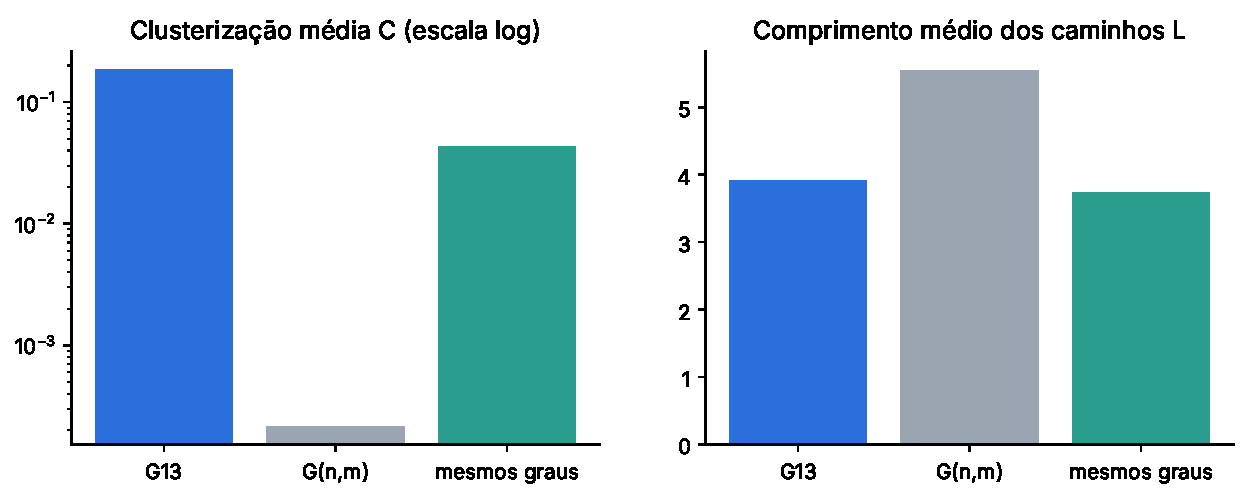
\includegraphics[width=\linewidth]{05_small_world.pdf}
  \caption{Clusterização e caminho médio do G13 e dos dois modelos nulos.}
  \label{fig:sw}
\end{figure}

\textbf{(2) Lei de potência.} O gráfico de $\log P(k)$ por $\log k$ é aproximadamente linear
(Figura~\ref{fig:potencia}), e todas as estimativas dão $\gamma > 1$ (Tabela~\ref{tab:potencia}).
A regressão sobre $P(k)$ bruto dá $\gamma = \gammaBruto$ ($R^2 = \rBruto$), mas é distorcida pela
cauda, onde muitos graus aparecem uma única vez. Com bins logarítmicos, $\gamma = \gammaBins$
($R^2 = \rBins$); por máxima verossimilhança, $\gamma = \gammaMLE$ para $k \geq \kminMLE$. A
distribuição é de cauda pesada, compatível com uma lei de potência com $2 < \gamma < 3$, longe da
Poisson esperada num grafo aleatório. A CCDF cai mais rápido no extremo da cauda, o que sugere um
corte para os maiores graus.

\begin{table}[t]
\centering
\small
\caption{Estimativas do expoente $\gamma$ da lei de potência.}
\label{tab:potencia}
\begin{adjustbox}{max width=\linewidth}
\begin{tabular}{lrr}
\toprule
 & $\gamma$ & $R^2$ / KS \\
\midrule
Regressão em $\log P(k)$ (bruto) & 1,44 & 0,861 \\
Regressão com bins logarítmicos & 2,11 & 0,992 \\
Regressão na CCDF & 2,32 & 0,962 \\
Máx. verossimilhança ($k_{min}=31$) & 2,22 & 0,0267 \\
\bottomrule
\end{tabular}
\end{adjustbox}
\end{table}


\begin{figure}[t]
  \centering
  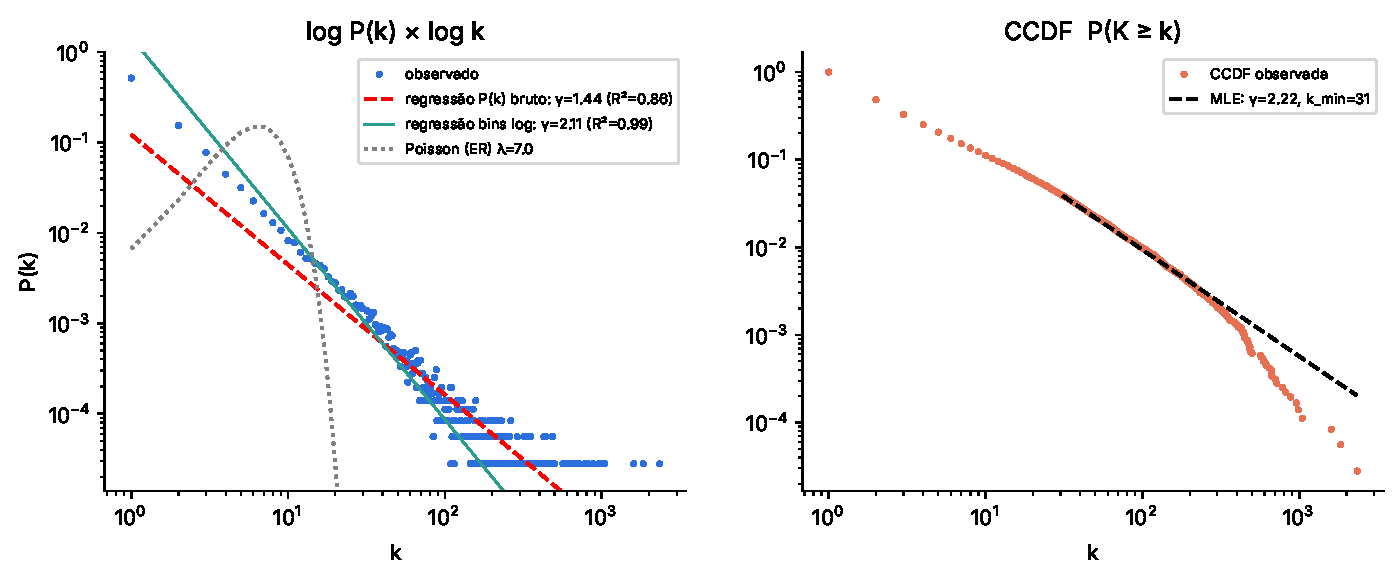
\includegraphics[width=\linewidth]{06_lei_potencia.pdf}
  \caption{Distribuição de graus em escala log-log com as retas ajustadas.}
  \label{fig:potencia}
\end{figure}

\textbf{(3) Robustez.} A Tabela~\ref{tab:robustez} e a Figura~\ref{fig:robustez} resumem as métricas A
a D. Com remoção aleatória de \rRemover{} vértices, a maior componente mantém \Srand{} dos vértices
originais ($\pm$\SrandDP), o caminho médio quase não muda (\Lrand{} contra \Lorig) e só \isoRand{}
dos vértices ficam isolados: a rede é robusta a falhas aleatórias. O ataque direcionado é devastador:
removendo os mesmos \rRemover{} vértices por grau, a maior componente cai para \Sgrau, o número de
componentes passa de 1 para \cgrau, o caminho médio triplica (\Lgrau) e \isoGrau{} dos vértices
restantes ficam isolados. O ataque por betweenness tem efeito quase igual ($S = \Sbtw$), e o por
PageRank é um pouco menos severo ($S = \Spr$), porque esse ranking privilegia subreddits muito citados
mesmo quando eles não são pontes entre regiões da rede. Como
$S_{rand} \gg S_{cent}$ e $c_{cent} \gg c_{rand}$, a rede é muito vulnerável a ataques direcionados,
o padrão de redes com hubs descrito por \citet{albert2000}.

\begin{table*}[t]
\centering
\small
\caption{Robustez da maior componente após remover $r=\lceil 0{,}05n \rceil$ vértices.}
\label{tab:robustez}
\begin{adjustbox}{max width=\linewidth}
\begin{tabular}{lrrrrr}
\toprule
 & $r$ & A: $S$ & B: $c$ & C: $L$ & D: isolados \\
\midrule
original & 0 & 1 & 1 & 3,92 & 0 \\
aleatória (média) & 1.734 & 0,924 & 869 & 3,92 & 0,0254 \\
aleatória (desvio) & 1.734 & 0,00457 & 155 & 0,0391 & 0,00462 \\
ataque por grau & 1.734 & 0,366 & 17.458 & 12,1 & 0,486 \\
ataque por betweenness & 1.734 & 0,364 & 17.799 & 8,7 & 0,498 \\
ataque por PageRank & 1.734 & 0,428 & 16.176 & 6,69 & 0,457 \\
\bottomrule
\end{tabular}
\end{adjustbox}
\end{table*}


\begin{figure*}[t]
  \centering
  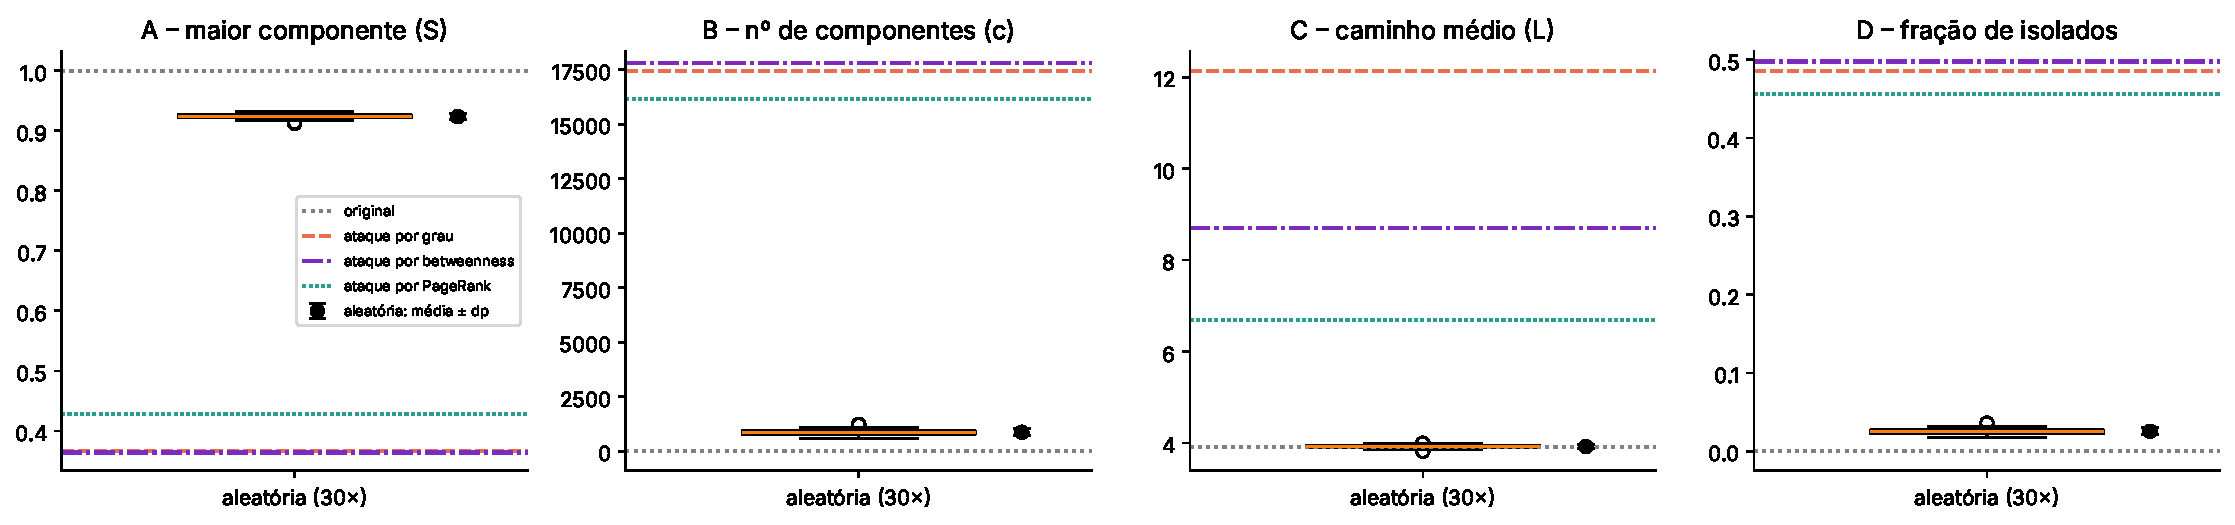
\includegraphics[width=\textwidth]{07_robustez.pdf}
  \caption{Métricas A a D: boxplot da remoção aleatória (30 repetições) e linhas dos ataques.}
  \label{fig:robustez}
\end{figure*}

\textbf{(4) Descoberta mais interessante.} Os links negativos são raros (\fracNeg) e muito
concentrados: 1\% dos subreddits que mais enviam links negativos responde por \concNeg{} deles
(Tabela~\ref{tab:negativos}). Quem mais ataca são comunidades de "meta-discussão" e drama
(\texttt{\topNeg}, \texttt{circlebroke}, \texttt{drama}), cujo propósito é comentar outras comunidades;
quem mais recebe são os grandes subreddits gerais (\texttt{askreddit}, \texttt{news},
\texttt{worldnews}). O perfil dos hubs (Tabela~\ref{tab:hubs}) mostra a mesma divisão: os hubs de
entrada (\texttt{\topIndegree}, \texttt{iama}, \texttt{pics}) são citados, os de saída citam. Isso
explica a baixa reciprocidade (\reciprocidade{} das arestas têm volta) e a maior componente fortemente
conexa pequena (\fracSCC): o conflito no Reddit flui de um pequeno grupo de comunidades
especializadas para as grandes vitrines da plataforma, e raramente volta.

\begin{table}[t]
\centering
\small
\caption{Subreddits que mais enviam e recebem links negativos (nº de posts).}
\label{tab:negativos}
\begin{adjustbox}{max width=\linewidth}
\begin{tabular}{rll}
\toprule
 & mais links negativos enviados & mais links negativos recebidos \\
\midrule
1 & subredditdrama (1437) & askreddit (892) \\
2 & circlebroke (702) & news (390) \\
3 & drama (518) & worldnews (390) \\
4 & shitliberalssay (407) & videos (373) \\
5 & circlejerkcopypasta (380) & pics (364) \\
6 & copypasta (372) & todayilearned (362) \\
7 & writingprompts (287) & funny (304) \\
8 & conspiracy (281) & adviceanimals (235) \\
9 & bestofoutrageculture (229) & relationships (216) \\
10 & karmacourt (210) & kotakuinaction (200) \\
\bottomrule
\end{tabular}
\end{adjustbox}
\end{table}

\begin{table*}[t]
\centering
\small
\caption{Perfil dos 10 subreddits de maior grau.}
\label{tab:hubs}
\begin{adjustbox}{max width=\linewidth}
\begin{tabular}{lrrrrrrrr}
\toprule
subreddit & grau & entrada & saída & PageRank & betweenness & recíproco & neg. enviados & neg. recebidos \\
\midrule
askreddit & 2.336 & 2.161 & 363 & 0,0164 & $7,07 \times 10^{7}$ & 0,0805 & 0,149 & 0,122 \\
iama & 1.839 & 1.646 & 384 & 0,0133 & $5,64 \times 10^{7}$ & 0,104 & 0,0254 & 0,049 \\
subredditdrama & 1.598 & 454 & 1.350 & 0,00153 & $4,27 \times 10^{7}$ & 0,129 & 0,308 & 0,177 \\
writingprompts & 1.043 & 717 & 426 & 0,00392 & $2,20 \times 10^{7}$ & 0,0959 & 0,168 & 0,0414 \\
outoftheloop & 986 & 592 & 507 & 0,00234 & $2,53 \times 10^{7}$ & 0,115 & 0,0705 & 0,0783 \\
pics & 956 & 953 & 4 & 0,00666 & $1,58 \times 10^{7}$ & 0,00105 & 0 & 0,131 \\
videos & 881 & 879 & 3 & 0,00844 & $2,21 \times 10^{7}$ & 0,00114 & 0 & 0,152 \\
todayilearned & 816 & 816 & 0 & 0,00465 & $1,23 \times 10^{7}$ & 0 & 0 & 0,153 \\
funny & 783 & 757 & 40 & 0,0039 & $1,16 \times 10^{7}$ & 0,0179 & 0,0909 & 0,149 \\
gaming & 719 & 584 & 226 & 0,00364 & $1,56 \times 10^{7}$ & 0,127 & 0,0632 & 0,0942 \\
\bottomrule
\end{tabular}
\end{adjustbox}
\end{table*}


\textbf{Extra: modelos clássicos.} A Tabela~\ref{tab:modelos} e a Figura~\ref{fig:modelos} comparam o
G13 a Erdős–Rényi, Barabási–Albert~\cite{barabasi1999} e Watts–Strogatz~\cite{watts1998}, gerados por
código próprio com o mesmo $n$ e $m$ aproximado. Nenhum reproduz tudo: o ER não tem hubs nem
agrupamento; o WS tem agrupamento, mas caminhos longos e graus homogêneos; o BA reproduz a cauda
pesada e os caminhos curtos, mas não a clusterização. O G13 combina a cauda do BA com um agrupamento
local que nenhum dos três gera.

\begin{table*}[t]
\centering
\small
\caption{G13 comparado aos modelos clássicos gerados com o mesmo $n$ e $m$ aproximado.}
\label{tab:modelos}
\begin{adjustbox}{max width=\linewidth}
\begin{tabular}{lrrrrrrrr}
\toprule
Modelo & n & m & grau máx & C médio & L & γ (bins log) & R² (bins log) & γ (MLE) \\
\midrule
G13 (maior componente) & 34.671 & 123.570 & 2.336 & 0,186 & 3,96 & 2,11 & 0,992 & 2,22 \\
Erdős–Rényi G(n,m) & 34.671 & 123.570 & 22 & $1,65 \times 10^{-4}$ & 5,52 & 1,46 & 0,195 & 2,92 \\
Barabási–Albert (m=4) & 34.671 & 138.668 & 620 & 0,00235 & 4,27 & 2,87 & 0,99 & 2,88 \\
Watts–Strogatz (k=8, p=0,1) & 34.671 & 138.684 & 12 & 0,473 & 8,07 & -5,03 & 0,361 & 5,71 \\
\bottomrule
\end{tabular}
\end{adjustbox}
\end{table*}


\begin{figure}[t]
  \centering
  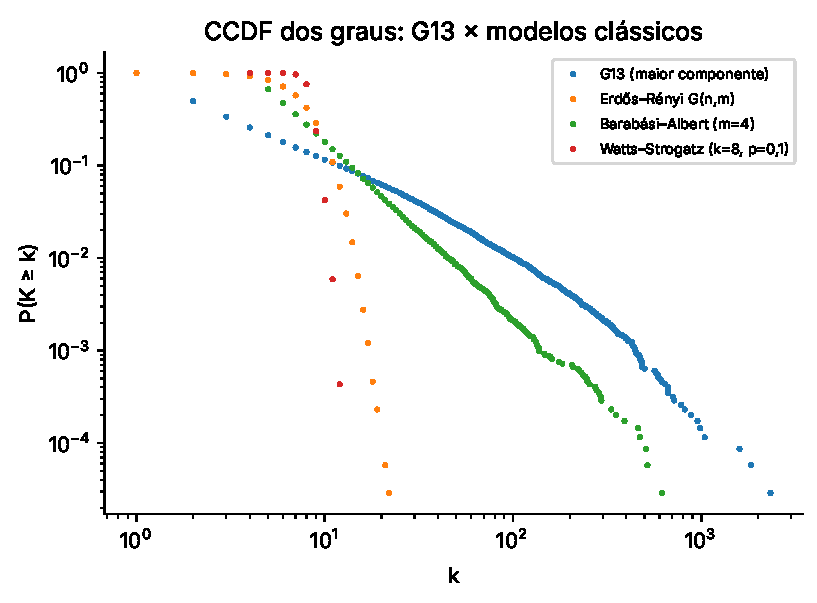
\includegraphics[width=\linewidth]{09_modelos_ccdf.pdf}
  \caption{CCDF dos graus do G13 e dos modelos clássicos.}
  \label{fig:modelos}
\end{figure}

% =================================================================================
\section{Discussão Crítica}
\textbf{Escolhas de tratamento.} Usamos apenas o arquivo \emph{body}; com o \emph{title}, o grafo teria
mais arestas, e as medidas mudariam em magnitude. A união temporal apaga a dinâmica: um link de 2014 e
um de 2017 pesam igual. O sinal majoritário resume pares com links dos dois tipos, e a conversão para
não dirigido perde a assimetria que, como vimos, é uma das características mais marcantes da rede.

\textbf{Aproximações.} O caminho médio, o diâmetro e o raio são exatos, mas o $L$ usado nas
comparações de small-world e de robustez é estimado por 200 a 300 BFS; o betweenness usa 1.000 das
\nLCC{} fontes (85\% dos vértices mais centrais coincidem com o valor exato). Os nulos aleatórios usam
poucas repetições, suficientes para diferenças da ordem das observadas, mas não para diferenças sutis.

\textbf{Lei de potência.} A forma da distribuição é compatível com uma lei de potência, mas não
fizemos o teste de hipótese de \citet{clauset2009} contra alternativas como a log-normal; o desvio na
cauda extrema indica que um corte exponencial pode descrever melhor os maiores graus.

\textbf{Tempos.} Os tempos dependem da máquina e do interpretador; o que importa é o crescimento.
Ainda assim, o ajuste $c \cdot f(n,m)$ mostrou que a forma dos subgrafos de teste influencia a curva
observada, e isso deve ser considerado ao ler qualquer análise de complexidade empírica.

% =================================================================================
\section{Conclusão}
A rede de hiperlinks entre subreddits é esparsa, quase conexa e de mundo pequeno: qualquer comunidade
está a cerca de quatro saltos de outra. A distribuição de graus tem cauda pesada ($\gamma \approx
\gammaMLE$), e essa estrutura de hubs a torna robusta a falhas aleatórias e muito frágil a ataques
direcionados. Os algoritmos implementados confirmaram as complexidades teóricas, com a ressalva de que
custos constantes por vértice pesam em Python. A descoberta mais interessante é a assimetria do conflito:
poucas comunidades de meta-discussão geram a maior parte dos links negativos, dirigidos às grandes
comunidades gerais, que raramente respondem. Trabalhos futuros podem incluir o arquivo \emph{title},
uma análise temporal e um teste formal da lei de potência.

\bibliographystyle{ACM-Reference-Format}
\bibliography{referencias}

\end{document}
